%%%%%%%%%%%%%%%%%%%%%%%%%%%%%%%%%%%%%%%%%%%%%%%%%%%%%%%%%%%%%%%%%%%%%%%%%%%%%%%%
%% Plantilla de memoria en LaTeX para la ETSIT - Universidad Rey Juan Carlos
%%
%% Por Gregorio Robles <grex arroba gsyc.urjc.es>
%%     Grupo de Sistemas y Comunicaciones
%%     Escuela Técnica Superior de Ingenieros de Telecomunicación
%%     Universidad Rey Juan Carlos
%% (muchas ideas tomadas de Internet, colegas del GSyC, antiguos alumnos...
%%  etc. Muchas gracias a todos)
%%
%% La última versión de esta plantilla está siempre disponible en:
%%     https://github.com/gregoriorobles/plantilla-memoria
%%
%% Para obtener PDF, ejecuta en la shell:
%%   make
%% (las imágenes deben ir en PNG o JPG)

%%%%%%%%%%%%%%%%%%%%%%%%%%%%%%%%%%%%%%%%%%%%%%%%%%%%%%%%%%%%%%%%%%%%%%%%%%%%%%%%

\documentclass[a4paper, 12pt]{book}
%\usepackage[T1]{fontenc}

\usepackage[a4paper, left=2.5cm, right=2.5cm, top=3cm, bottom=3cm]{geometry}
\usepackage{times}
\usepackage[utf8]{inputenc}
%\usepackage[latin1]{inputenc}
%\usepackage[spanish]{babel} % Comenta esta l�nea si tu memoria es en ingl�s
\usepackage{url}
%\usepackage[dvipdfm]{graphicx}
\usepackage{graphicx}
\usepackage{float}  %% H para posicionar figuras
\usepackage[nottoc, notlot, notlof, notindex]{tocbibind} %% Opciones de �ndice
\usepackage{latexsym}  %% Logo LaTeX
\usepackage{csquotes}  %% Paquete para citas (displayquote)
\usepackage{color}  %% Paquete para texto en color

\title{Memoria del Proyecto}
\author{Miguel Ángel Fernández Sánchez}

\renewcommand{\baselinestretch}{1.5}  %% Interlineado

\begin{document}

%\renewcommand{\refname}{Bibliografía}  %% Renombrando
%\renewcommand{\appendixname}{Apéndice}

%%%%%%%%%%%%%%%%%%%%%%%%%%%%%%%%%%%%%%%%%%%%%%%%%%%%%%%%%%%%%%%%%%%%%%%%%%%%%%%%
% PORTADA

\begin{titlepage}
\begin{center}
\begin{tabular}[c]{c c}
%\includegraphics[bb=0 0 194 352, scale=0.25]{logo} &
\includegraphics[scale=0.25]{img/logo_vect.png} &
\begin{tabular}[b]{l}
\Huge
\textsf{UNIVERSIDAD} \\
\Huge
\textsf{REY JUAN CARLOS} \\
\end{tabular}
\\
\end{tabular}

\vspace{3cm}

\Large
GRADO INGENIERÍA SISTEMAS AUDIOVISUALES Y MULTIMEDIA

\vspace{0.4cm}

\large
Curso Académico 2017/2018

\vspace{0.8cm}

Trabajo Fin de Grado

\vspace{2.5cm}

\LARGE
HERRAMIENTA PARA ANALIZAR PROYECTOS FLOSS EN GITHUB (prov.)
% http://dl.acm.org/citation.cfm?id=2976778
\vspace{4cm}

\large
Autor : Miguel Ángel Fernández Sánchez \\
Tutor : Dr. Gregorio Robles
\end{center}
\end{titlepage}

\newpage
\mbox{}
\thispagestyle{empty} % para que no se numere esta pagina


%%%%%%%%%%%%%%%%%%%%%%%%%%%%%%%%%%%%%%%%%%%%%%%%%%%%%%%%%%%%%%%%%%%%%%%%%%%%%%%%
%%%% Para firmar
\clearpage
\pagenumbering{gobble}
\chapter*{Evaluation}

\vspace{-4cm}
\begin{center}
\LARGE
\textbf{Trabajo Fin de Grado}

\vspace{1cm}
\large
Herramienta para la extracción y el análisis de proyectos FLOSS en GitHub (provisional)

\vspace{1cm}
\large
\textbf{Autor :} Miguel Ángel Fernández Sánchez \\
\textbf{Tutor :} Dr. Gregorio Robles Martínez

\end{center}

\vspace{1cm}
La defensa del presente Trabajo Fin de Grado se realizó el día \qquad$\;\,$ de \qquad\qquad\qquad\qquad \newline de 20XX, siendo calificada por el siguiente tribunal:


\vspace{0.5cm}
\textbf{Presidente:}

\vspace{1.2cm}
\textbf{Secretario:}

\vspace{1.2cm}
\textbf{Vocal:}


\vspace{1.2cm}
y habiendo obtenido la siguiente calificación:

\vspace{1cm}
\textbf{Calificación:}


\vspace{1cm}
\begin{flushright}
Fuenlabrada, a \qquad$\;\,$ de \qquad\qquad\qquad\qquad de 20XX
\end{flushright}

%%%%%%%%%%%%%%%%%%%%%%%%%%%%%%%%%%%%%%%%%%%%%%%%%%%%%%%%%%%%%%%%%%%%%%%%%%%%%%%%
%%%% Dedicatoria

\chapter*{Dedications}
\pagenumbering{Roman} % para comenzar la numeracion de paginas en numeros romanos
\begin{flushright}
\textit{Dedicado a \\
mi familia / mi abuelo / mi abuela}
\end{flushright}

%%%%%%%%%%%%%%%%%%%%%%%%%%%%%%%%%%%%%%%%%%%%%%%%%%%%%%%%%%%%%%%%%%%%%%%%%%%%%%%%
%%%% Agradecimientos

\chapter*{Acknowledgements}
%\addcontentsline{toc}{chapter}{Agradecimientos} % si queremos que aparezca en el �ndice
\markboth{AGRADECIMIENTOS}{AGRADECIMIENTOS} % encabezado

Aquí vienen los agradecimientos\ldots Aunque esté bien acordarse de la pareja,
no hay que olvidarse de dar las gracias a tu madre, que aunque a veces no lo
parezca disfruta tanto de tus logros como tú\ldots Además, la pareja quizás
no sea para siempre, pero tu madre sí.


%%%%%%%%%%%%%%%%%%%%%%%%%%%%%%%%%%%%%%%%%%%%%%%%%%%%%%%%%%%%%%%%%%%%%%%%%%%%%%%%
%%%% Resumen en ingl�s

\chapter*{Summary}
%\addcontentsline{toc}{chapter}{Summary} % si queremos que aparezca en el �ndice
\markboth{SUMMARY}{SUMMARY} % encabezado

Here comes a translation of the ``Resumen'' into English. Please, double check
it for correct grammar and spelling. As it is the translation of the ``Resumen'',
which is supposed to be written at the end, this as well should be filled out
just before submitting.


%%%%%%%%%%%%%%%%%%%%%%%%%%%%%%%%%%%%%%%%%%%%%%%%%%%%%%%%%%%%%%%%%%%%%%%%%%%%%%%%
%%%% Resumen

\chapter*{Resumen}
%\addcontentsline{toc}{chapter}{Resumen} % si queremos que aparezca en el �ndice
\markboth{RESUMEN}{RESUMEN} % encabezado

Aquí viene un resumen del proyecto. Ha de constar de tres o cuatro párrafos,
donde se presente de manera clara y concisa de qué va el proyecto. Han
de quedar respondidas las siguientes preguntas:

\begin{itemize}
  \item ¿De qué va este proyecto? ¿Cuál es su objetivo principal?
  \item ¿Cómo se ha realizado? ¿Qué tecnologías están involucradas?
  \item ¿En qué contexto se ha realizado el proyecto? ¿Es un proyecto
dentro de un marco general?
\end{itemize}
Lo mejor es escribir el resumen al final.
%%%%%%%%%%%%%%%%%%%%%%%%%%%%%%%%%%%%%%%%%%%%%%%%%%%%%%%%%%%%%%%%%%%%%%%%%%%%%%%%
%%%%%%%%%%%%%%%%%%%%%%%%%%%%%%%%%%%%%%%%%%%%%%%%%%%%%%%%%%%%%%%%%%%%%%%%%%%%%%%%
% �NDICES %
%%%%%%%%%%%%%%%%%%%%%%%%%%%%%%%%%%%%%%%%%%%%%%%%%%%%%%%%%%%%%%%%%%%%%%%%%%%%%%%%

% Las buenas noticias es que los �ndices se generan autom�ticamente.
% Lo �nico que tienes que hacer es elegir cu�les quieren que se generen,
% y comentar/descomentar esa instrucci�n de LaTeX.

%%%% �ndice de contenidos
\tableofcontents
%%%% �ndice de figuras
\cleardoublepage
%\addcontentsline{toc}{chapter}{Lista de figuras} % para que aparezca en el indice de contenidos
\listoffigures % indice de figuras
%%%% �ndice de tablas
%\cleardoublepage
%\addcontentsline{toc}{chapter}{Lista de tablas} % para que aparezca en el indice de contenidos
%\listoftables % indice de tablas


%%%%%%%%%%%%%%%%%%%%%%%%%%%%%%%%%%%%%%%%%%%%%%%%%%%%%%%%%%%%%%%%%%%%%%%%%%%%%%%%
%%%%%%%%%%%%%%%%%%%%%%%%%%%%%%%%%%%%%%%%%%%%%%%%%%%%%%%%%%%%%%%%%%%%%%%%%%%%%%%%
% INTRODUCCI�N %
%%%%%%%%%%%%%%%%%%%%%%%%%%%%%%%%%%%%%%%%%%%%%%%%%%%%%%%%%%%%%%%%%%%%%%%%%%%%%%%%

\cleardoublepage
\chapter{Introduction}
\label{sec:intro} % etiqueta para poder referenciar luego en el texto con ~\ref{sec:intro}
\pagenumbering{arabic} % para empezar la numeraci�n de p�gina con n�meros
% En este cap�tulo se introduce el proyeto. Deber�a tener informaci�n general sobre
% el mismo, dando la informaci�n sobre el contexto en el �que se ha desarrollado.
% No te olvides de echarle un ojo a la p�gina con los cinco errores de escritura m�s frecuentes\footnote{\url{http://www.tallerdeescritores.com/errores-de-escritura-frecuentes}}.
% #TODO Ask for resources to back this data:
The way people develop software has evolved during these years: there is an extended social perception of developers to
being ingoing, solitary people, with very few social skills. But this sense is outdated: the paradigm has changed,
as coding has become almost a social activity. Developers who work collaborating with others produce better software [resource], as they
are continuously reading code from other developers, getting feedback about their contributions and consequently
widening their knowledge with new procedures and ideas. It turns out that this is how most of the software is produced nowadays,
so it is very difficult to become a successful developer without having good social skills.\\
If we think on social, virtual interactions among people, the first thing that probably come to our minds will be
"Social networks". It is clear that those so-called social networks have produced a huge impact among a big part of the
population; changing daily habits, affecting real-life relationships, etc. As individuals, we share personal information every
day using interactive applications which allows us to participate somehow into a social network. Because of handling these
applications, we make specific interactions as users. \\
Let's see some examples. If we focus on Twitter, some of these interactions can be:
\begin{itemize}
    \item Follow a Twitter user.
    \item \textit{Retweet} a \textit{tweet} (propagate a message among all followers of the person who \textit{retweetted}).
    \item Use a \textit{hashtag} (a word preceded by a hash \# to label or classify a message into a topic).
\end{itemize}
\pagebreak Whereas on Facebook, we have other kinds of interactions:
\begin{itemize}
    \item React to a post.
    \item Tag a person in a picture.
    \item Write a comment on someone's profile.
\end{itemize}
Talking about coding, in the last few years we've seen how this social trend came to software with the
emergence of social coding platforms, such as GitHub, BitBucket, GitLab, etc.\\
Social interactions in these platforms are about how software is developed and maintained but also how
contributions are managed (code review, continuous integration, etc.).\\
So, for example, on GitHub\footnote{\url{https://github.com}} we can find interactions like:
\begin{itemize}
    \item \textit{Fork} a repository (create an editable copy of a project).
    \item See changes from last \textit{commit} (difference between most recent version and last version of the project).
    \item Check the contributors of a repository.
    \item Submit a \textit{Pull Request} (proposal to merge changes in a project).
\end{itemize}
These interactions that were mentioned, no matter their source, leave traces which remain stored in some computer on Earth.
This means we can obtain these data (though not all of it is publicly available) through the Internet using an \emph{API}
(\textit{Application programming interface}).\\
Once this information is retrieved, we can analyze it and extract conclusions about it.

\section{Free/Libre/Open-Source Software}
\label{sec:floss-definition}
In the following sections, we are going to talk about software and its development process, focusing on \emph{FLOSS} (Free/Libre, Open-source
software) projects, so it is inevitable to describe briefly what is this about.
During my degree, I was fortunate to be taught within \emph{FLOSS} values, as most of my professors plead
for Free/Libre software as their teaching model, by which I have obtained a distinctive knowledge and perspective as a professional but also as an individual.\\
\newpage
According to the \textbf{Free Software Foundation}\footnote{\url{https://www.gnu.org/philosophy/free-sw.html}}:
\begin{displayquote}
    \emph{Free software} means software that respects users' freedom and community. Roughly, it means that the users have the freedom
    to run, copy, distribute, study, change and improve the software. Thus, free software is a matter of liberty, not price. (\ldots)\\
    A program is free software if the program's users have the four essential freedoms:
       \begin{itemize}
           \item The freedom to run the program as you wish, for any purpose (freedom 0).
           \item The freedom to study how the program works, and change it so it does your computing as you wish (freedom 1).
           \item The freedom to redistribute copies (freedom 2).
           \item The freedom to distribute copies of your modified versions to others (freedom 3).
       \end{itemize}
    A program is free software if it gives users adequately all of these freedoms. Otherwise, it is \textit{nonfree}.
\end{displayquote}
% #TODO:
Due to the connotations which the word \emph{Free} has in English language (mentioned before), there is a definition
for \emph{Open source} software by the \textbf{Open Source Initiative}\footnote{\url{https://opensource.org/osd}} which
slighly varies from the \emph{FSF} definition. About this difference, Richard Stallman (founder of the \emph{FSF}) comments:
\begin{displayquote}
The term \emph{open source} software is used by some people to mean more or less the same category as free software.
It is not exactly the same class of software: they accept some licenses that we consider too restrictive,
and there are free software licenses they have not accepted. However, the differences in extension of the
category are small: nearly all free software is open source, and nearly all open source software is free.
\end{displayquote}
%Example code: \begin{verbatim}
\section{Motivation}
\label{sec:motivation}
I was working as a Researcher Assistant in \emph{GSyC/LibreSoft}\footnote{\url{http://www.libresoft.es}} department at Rey Juan Carlos University when I started to
deepen into Free/Libre software and the world of metrics. Then I had the great luck of start participating in a study that
Dr. Gregorio Robles was doing with researchers from Chalmers University in Gothenburg, Sweden. The main aim of their research was to
learn how \emph{UML} models\footnote{\url{http://uml.org/what-is-uml.htm}} are used in public \emph{FLOSS} projects (particularly, projects hosted on GitHub),
as most of the previous studies focused only on its industrial use.\\
Given the large size of GitHub as a platform and its access limitations, this research motivated to build a tool which extracts
data from all the existing repositories on GitHub, then filter those repositories which may include at least one
\emph{UML} model and finally analyze more in-depth the set of projects that meet this condition.\\\\
Since early stages of this research, this tool was designed and built using a modular structure, thought to be reusable
and adaptable to any kind of files that have to be found but also the way GitHub provides data; hoping to be useful
for other researches or any other person who might be interested on extract this information. Besides, the scale of this project
presented a personal challenge which provided me the opportunity to extend my knowledge and obtain a valuable point of
view about research and large-scope projects.
\section{Structure of the dissertation}
\label{sec:estructura}
\textcolor{red}{(Work in progress)}\newline
During this dissertation, I'm going to explain the different objectives that were stated for this project, the technology
which have been used to make it happen.\\
After that, I'll detail the designing process and the tool architecture, itemizing on each one of its sections. Then,
we'll explore the performance of the tool within a use case, taking into account the limitations and issues which arose
during it and how they were solved.\\Then, discuss about results from the use case and general conclusions
and to finish, consider future work and further steps for this project.
%%%%%%%%%%%%%%%%%%%%%%%%%%%%%%%%%%%%%%%%%%%%%%%%%%%%%%%%%%%%%%%%%%%%%%%%%%%%%%%%
%%%%%%%%%%%%%%%%%%%%%%%%%%%%%%%%%%%%%%%%%%%%%%%%%%%%%%%%%%%%%%%%%%%%%%%%%%%%%%%%
% OBJETIVOS %
%%%%%%%%%%%%%%%%%%%%%%%%%%%%%%%%%%%%%%%%%%%%%%%%%%%%%%%%%%%%%%%%%%%%%%%%%%%%%%%%
\cleardoublepage
\chapter{Objectives}
\label{chap:objetivos}
It is widely known that \emph{GitHub} allows to filter projects by a certain programming language (e.g.
\emph{Python}, \emph{C++}, etc.), but \emph{GitHub} does not offer a mechanism through which you can identify projects
containing files with a certain extension or how many files match with some word or pattern in their
filename in a repository. The fundamental research questions that motivated the creation of this tool were:
\begin{itemize}
  \item RQ1: How many \emph{GitHub} repositories contain at least one file with a certain extension or a certain
        pattern in its filename?
  \item RQ2: What's the history of those files in the life-span of the project?
\end{itemize}
Therefore, the main goal of this tool is to extract and analyse data from a set of GitHub projects in a scalable,
automated way in order to obtain quantitative information about the usage of a certain file type, programming language
or/and any search that can be expressed into patterns and heuristics.\\\\
Thus far, many studies focused in one single project or in a limited dataset when software development is analyzed, so
the next goal to define is to obtain the whole dataset of repositories hosted on all \emph{GitHub} at a certain date.\\
For analyze the data from all \emph{GitHub} in a proper way, we needed an static, reliable and updated source of this platform.\
This source is produced by the \emph{GHTorrent} project by a queriable, offline database with most of the information which the
\emph{GitHub} \textit{API} can provide.\\
To finish answering \emph{RQ1}, we need to extract the list of files from the main branch [definition] of each repository so
it can be applied the different filters.\\\\
To answer to \emph{RQ2}, we need to analyze more in-depth marking those repositories with at least one positive result
after applying the filter, and then build a database with this extended data to extract useful information from it in a
systematic way.
%%%%%%%%%%%%%%%%%%%%%%%%%%%%%%%%%%%%%%%%%%%%%%%%%%%%%%%%%%%%%%%%%%%%%%%%%%%%%%%%
%%%%%%%%%%%%%%%%%%%%%%%%%%%%%%%%%%%%%%%%%%%%%%%%%%%%%%%%%%%%%%%%%%%%%%%%%%%%%%%%
% ESTADO DEL ARTE %
%%%%%%%%%%%%%%%%%%%%%%%%%%%%%%%%%%%%%%%%%%%%%%%%%%%%%%%%%%%%%%%%%%%%%%%%%%%%%%%%
\cleardoublepage
\chapter{State of the art}
%Puedes citar libros, como el de Bonabeau et al. sobre procesos estigm�rgicos~\cite{bonabeau:_swarm}.
 % Nota que el ~ a�ade un espacio en blanco, pero no deja que exista un salto de l�nea. Imprescindible ponerlo para las citas.
\section{Python}
\label{sec:python}
\textbf{Python}\footnote{\url{https://www.python.org/}} is an interpreted, object-oriented, high-level, open source
programming language for general-purpose programming created by Guido van Rossum in 1991 (Nowadays, the most
recent version is 3.6.4, from December, 2017).\ Its design is focused on code readability and clear syntax, making
possible to program using fewer lines of code comparing to other programming languages as \emph{C++} or \emph{Ada}.\\
%Python is widely used over the world, for example: Numeric and Scientific Programming, ... \\
\emph{Python} features a large standard library, which includes many different tasks from text pattern matching to network
scripting, in addition to a vast collection of third-party application libraries.
Other remarkable features are portability, as \emph{Python} interpreters are available for many operating systems;
and the component integration, as \emph{Python} scripts can easily communicate with other parts of an application or code,
like \emph{C++} libraries, \emph{MySQL} databases, etc.\\
%As a downside to Python is that its execution speed may not always be as fast as a compiled, lower-level
%slanguages such as C and C++.\\
\section{Git}
\label{sec:git}
%source: https://git-scm.com/book/en/v2/Getting-Started-Git-Basics
\textbf{Git} is an open-source Version Control System (\emph{VCS}), originally developed in 2005 by Linus Torvalds.\
As any \emph{VCS}, \emph{Git} is a system that records changes to a file or set of files over time
so that you can recall specific versions later.
It's by far, the most used \emph{VCS} in the world\footnote{\url{http://stackoverflow.com/research/developer-survey-2015}}.\\\\
The major difference between \emph{Git} and any other VCS is the way \emph{Git} thinks about its data.
Conceptually, most other systems store information as a list of file-based changes. Other systems like \textit{Subversion},
\textit{Perforce}, \textit{Bazaar}, etc. think of the information they store as a set of files and the changes made to each
file over time.\\
Instead, \emph{Git} thinks of its data more like a series of snapshots of a miniature filesystem.
With \emph{Git}, every time you commit or save the state of your project, \emph{Git} basically takes a picture of what all
your files look like at that moment and stores a reference to that snapshot. To be efficient, if files have not changed,
\emph{Git} doesn't store the file again, just a link to the previous identical file it has already stored.
\section{GitHub}
\label{sec:github}
\textbf{GitHub} is a \emph{Git}, web-based repository hosting service founded back in 2008. While \emph{Git} is a command
line tool, \emph{GitHub} provides a graphical interface, adding its own collaboration features such as a wikis and basic task
management tools for every project.\\
Each user on \emph{GitHub} has their own profile, showing its past work and contributions to
other projects via \textit{pull requests}, \textit{forking} (create editable copies into someone's account) other repositories, etc.
Project revisions can be discussed publicly via \textit{issues} so many people can collaborate together to advance a project
forward. Currenty, \emph{GitHub} is the largest host of source code in the world,
with more than 124 million projects.
% TODO: https://www.quora.com/How-many-repositories-are-there-on-GitHub
%       https://www.howtogeek.com/180167/htg-explains-what-is-github-and-what-do-geeks-use-it-for/
%       https://techcrunch.com/2012/07/14/what-exactly-is-github-anyway/
\subsection{GitHub API}
\label{sec_gh-api}
%Should this definition be within a Glossary?
An \textbf{API} (\textit{Application Programming Interface}) is a set of subroutine definitions, protocols, and tools for building
application software. In general terms, it is a set of clearly defined methods of communication between various software components.\\\\
\emph{GitHub} \textit{API} allows to access GitHub data, since own \emph{GitHub} types like \textit{pull-requests}, \textit{issues} or \textit{forks}
to \emph{Git}-related data, such as \textit{commits}, \textit{branches} or \textit{trees} using \textit{HTTP} requests and
returning information using \emph{JSON}(\textit{JavaScript Object Notation}) format.
\section{GHTorrent}
\label{sec:ghtorrent}
\textbf{GHTorrent} is a project based on create a scalable, queriable, offline mirror of data offered through the \emph{GitHub} \textit{API}.\\
As they explain in their website\footnote{\url{http://ghtorrent.org/}}, \emph{GHTorrent} monitors the \emph{GitHub} public event time line.
For each event, it retrieves its contents and their dependencies, exhaustively. Then, it stores the raw responses to a \emph{MongoDB} database.
database, while also extracting their structure in a MySQL database.\
For each release, you can choose the \textit{dump} (a raw copy of a database) you want to download: either a \emph{MySQL} dump
(the full database, using one file per table) or a \emph{MongoDB} one (an incremental database).\\
\section{GrimoireLab and Perceval}
\label{sec:grimoire}
\textbf{GrimoireLab}\footnote{\url{http://grimoirelab.github.io/}} is a free, open source toolset for software development analytics
mainly developed by the Spanish company \emph{Bitergia}\footnote{\url{https://bitergia.com/}}.
It allows you to retrieve data from many kinds of systems with information related to software development, and produce
analysis and visualizations with it.\\
We are focusing on a particular tool of \emph{GrimoireLab} called \textbf{Perceval}. This tool can retrieve data from more
than 20 different kinds of data sources, from \emph{git} repositories or \emph{GitHub} projects, to issue trackers such as \emph{Jira}
or \emph{Bugzilla}, including messaging systems such as \emph{IRC}, \emph{Slack} or mailing lists, or other types of systems such as
\emph{StackOverflow} or \emph{Jenkins} in a regular and incremental way, allowing to produce uniform sets of information.
\newline \emph{GrimoireLab} is now part of \emph{CHAOSS}\footnote{\url{https://chaoss.community/}}, a project by \emph{The Linux Foundation}.
%%%%%%%%%%%%%%%%%%%%%%%%%%%%%%%%%%%%%%%%%%%%%%%%%%%%%%%%%%%%%%%%%%%%%%%%%%%%%%%%
%%%%%%%%%%%%%%%%%%%%%%%%%%%%%%%%%%%%%%%%%%%%%%%%%%%%%%%%%%%%%%%%%%%%%%%%%%%%%%%%
% DISEÑO E IMPLEMENTACIÓN %
%%%%%%%%%%%%%%%%%%%%%%%%%%%%%%%%%%%%%%%%%%%%%%%%%%%%%%%%%%%%%%%%%%%%%%%%%%%%%%%%
\cleardoublepage
\chapter{Design and implementation}
\section{General architecture}
\label{sec:arquitectura}
This tool has a modular design, to ease its adaptability to future updates, changes on it dependencies or other needs which may appear.
The tool is divided into several sections with a set of Python scripts, which can be grouped into three
main phases (See figure~\ref{fig:arquitectura}).
\begin{figure}
  \centering
  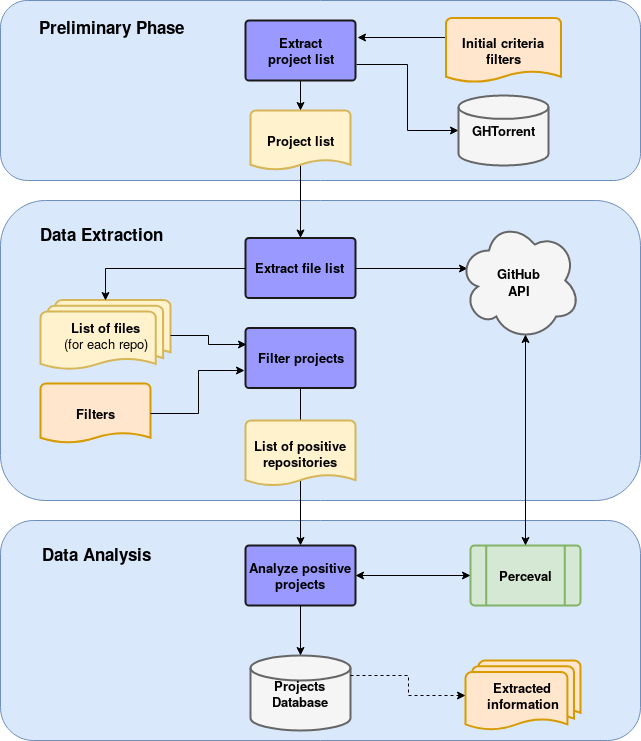
\includegraphics[width=12cm, keepaspectratio]{img/generic-tool-diagram-sections}
  \caption{General architecture of the tool}
  \label{fig:arquitectura}
\end{figure}
Before going into detail in each of these stages, let's introduce them briefly:
\begin{enumerate}
  \item \textbf{Preliminary phase}
    \begin{itemize}
      \item \textbf{Extract project list}:
            In this preliminary phase is where the list of GitHub repositories is retrieved. Using an offline dump of
            the \emph{GHTorrent} database, we get the file containing all GitHub repositories from one of its tables
            and use a filter to choose among projects by their fields, like a major programming language,
            \textit{forked} or not, etc.
    \end{itemize}
  \item \textbf{Data extraction}
    \begin{itemize}
      \item \textbf{Extract file list}:
            This is the most critical section, because is where we obtain the main \textit{branch} and the file list
            (for each repository in the list from last section) quering the \emph{GitHub} \textit{API}.
      \item \textbf{Filter projects}:
            It consists on iterating over the extracted file lists applying the corresponding patterns and heuristics.
            Then, a file is produced with the positive results (repositories with at least one match).
    \end{itemize}
  \item \textbf{Data analysis}
    \begin{itemize}
      \item \textbf{Analyze positive projects}:
            Its function is to execute \emph{Perceval} with every project on the list of positive repositories
            building a database which can be queried to extract information.
    \end{itemize}
\end{enumerate}
\section{Preliminary phase}
\label{sec:fase-preliminar}
\section{Data extraction}
\label{sec:extraccion-datos}
\section{Data filtering}
\label{sec:filtro-datos}
\section{Data analysis}
\label{sec:analisis-datos}
%%%%%%%%%%%%%%%%%%%%%%%%%%%%%%%%%%%%%%%%%%%%%%%%%%%%%%%%%%%%%%%%%%%%%%%%%%%%%%%%
%%%%%%%%%%%%%%%%%%%%%%%%%%%%%%%%%%%%%%%%%%%%%%%%%%%%%%%%%%%%%%%%%%%%%%%%%%%%%%%%
% RESULTADOS %
%%%%%%%%%%%%%%%%%%%%%%%%%%%%%%%%%%%%%%%%%%%%%%%%%%%%%%%%%%%%%%%%%%%%%%%%%%%%%%%%
\cleardoublepage
\chapter{Results}
\section{Case of study: UML}
\label{sec:caso-estudio-uml}
%%%%%%%%%%%%%%%%%%%%%%%%%%%%%%%%%%%%%%%%%%%%%%%%%%%%%%%%%%%%%%%%%%%%%%%%%%%%%%%%
%%%%%%%%%%%%%%%%%%%%%%%%%%%%%%%%%%%%%%%%%%%%%%%%%%%%%%%%%%%%%%%%%%%%%%%%%%%%%%%%
% CONCLUSIONES %
%%%%%%%%%%%%%%%%%%%%%%%%%%%%%%%%%%%%%%%%%%%%%%%%%%%%%%%%%%%%%%%%%%%%%%%%%%%%%%%%
\cleardoublepage
\chapter{Conclusions}
\label{chap:conclusiones}
\section{Achieved objectives}
\label{sec:consecucion-objetivos}
Esta sección es la sección espejo de las dos primeras del capítulo de objetivos,
donde se planteaba el objetivo general y se elaboraban los específicos.
Es aquí donde hay que debatir qué se ha conseguido y qué no. Cuando algo no
se ha conseguido, se ha de justificar, en términos de qué problemas se han
encontrado y qué medidas se han tomado para mitigar esos problemas.
\section{Knowledge application}
\label{sec:aplicacion}
Aquí viene lo que has aprendido durante el Grado/Máster y que has aplicado
en el TFG/TFM. Una buena idea es poner las asignaturas más relacionadas y
comentar en un párrafo los conocimientos y habilidades puestos en práctica.
\subsection{Related courses}
\begin{itemize}
  \item Informática 1
  \item Informática 2
  \item Arquitectura de Internet
  \item Sistemas Telemáticos para medios audiovisuales
  \item Protocolos de Transmisión de Audio y Video en Internet
  \item Laboratorio de Tecnologías Audiovisuales en la Web
\end{itemize}
\section{Learning outcomes}
\label{sec:lecciones_aprendidas}
Aquí viene lo que has aprendido en el Trabajo Fin de Grado/Máster.
\begin{enumerate}
  \item a
  \item b
\end{enumerate}
\section{Future work}
\label{sec:trabajos_futuros}
Ningún software se termina, así que aquí vienen ideas y funcionalidades
que estaría bien tener implementadas en el futuro.
Es un apartado que sirve para dar ideas de cara a futuros TFGs/TFMs.
\section{Personal assessment}
\label{sec:valoracion}
Finalmente (y de manera opcional), hay gente que se anima a dar su punto de
vista sobre el proyecto, lo que ha aprendido, lo que le gustaría haber aprendido,
las tecnologías utilizadas y demás.
%%%%%%%%%%%%%%%%%%%%%%%%%%%%%%%%%%%%%%%%%%%%%%%%%%%%%%%%%%%%%%%%%%%%%%%%%%%%%%%%
%%%%%%%%%%%%%%%%%%%%%%%%%%%%%%%%%%%%%%%%%%%%%%%%%%%%%%%%%%%%%%%%%%%%%%%%%%%%%%%%
% AP�NDICE(S) %
%%%%%%%%%%%%%%%%%%%%%%%%%%%%%%%%%%%%%%%%%%%%%%%%%%%%%%%%%%%%%%%%%%%%%%%%%%%%%%%%
\cleardoublepage
\appendix
\chapter{User manual}
\label{app:manual}
\chapter{Published papers}
\label{app:papers}
%%%%%%%%%%%%%%%%%%%%%%%%%%%%%%%%%%%%%%%%%%%%%%%%%%%%%%%%%%%%%%%%%%%%%%%%%%%%%%%%
%%%%%%%%%%%%%%%%%%%%%%%%%%%%%%%%%%%%%%%%%%%%%%%%%%%%%%%%%%%%%%%%%%%%%%%%%%%%%%%%
% BIBLIOGRAFIA %
%%%%%%%%%%%%%%%%%%%%%%%%%%%%%%%%%%%%%%%%%%%%%%%%%%%%%%%%%%%%%%%%%%%%%%%%%%%%%%%%
\cleardoublepage
% Las siguientes dos instrucciones es todo lo que necesitas
% para incluir las citas en la memoria
\bibliographystyle{abbrv}
\bibliography{memoria}  % memoria.bib es el nombre del fichero que contiene
% las referencias bibliogr�ficas. Abre ese fichero y mira el formato que tiene,
% que se conoce como BibTeX. Hay muchos sitios que exportan referencias en
% formato BibTeX. Prueba a buscar en http://scholar.google.com por referencias
% y ver�s que lo puedes hacer de manera sencilla.
% M�s informaci�n:
% http://texblog.org/2014/04/22/using-google-scholar-to-download-bibtex-citations/
\end{document}
